% Created 2012-10-10 Wed 14:00
\documentclass[bigger]{beamer}
\usepackage[utf8]{inputenc}
\usepackage[T1]{fontenc}
\usepackage{fixltx2e}
\usepackage{graphicx}
\usepackage{longtable}
\usepackage{float}
\usepackage{wrapfig}
\usepackage{soul}
\usepackage{textcomp}
\usepackage{marvosym}
\usepackage{wasysym}
\usepackage{latexsym}
\usepackage{amssymb}
\usepackage{hyperref}
\tolerance=1000
\titlegraphic{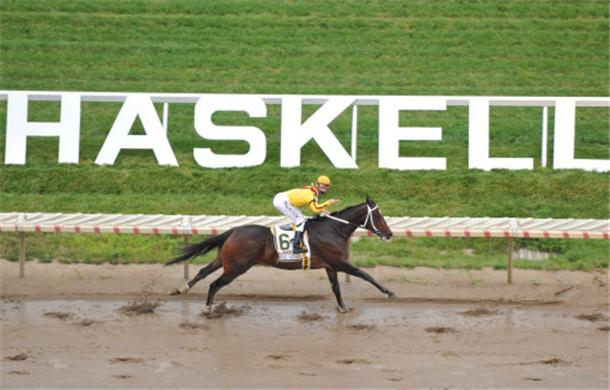
\includegraphics{../pictures/haskell_horse.jpg}}
\setbeamertemplate{navigation symbols}{}
\mode<beamer>{\usetheme{CambridgeUS}}
\institute{GWU}
\providecommand{\alert}[1]{\textbf{#1}}

\title{The Pony Project}
\author{Andrew Hirsch}
\date{2012-10-10 Wed}

\begin{document}

\maketitle


\begin{frame}
\frametitle{What Pony Is}
\label{sec-1}


\begin{itemize}
\item Pony is an extensible compiler
\item For C99
\item Written in Haskell
\begin{itemize}
\item A purely functional language
\end{itemize}
\end{itemize}
\end{frame}
\begin{frame}
\frametitle{What Already Exists}
\label{sec-2}


\begin{itemize}
\item Parts of Pony already exist
\begin{itemize}
\item Transformation data type
\item C Abstract Syntax Tree
\item Application of transformations
\end{itemize}
\item What doesn't exist
\begin{itemize}
\item An extensible parser 
    
    Can't parse anything that doesn't look like C!
\item Collision Detection
    
    When do two transformations cause a problem?
\item A Transformation Language
    
    Currently, a transformation writer must know Haskell
\end{itemize}
\end{itemize}
\end{frame}
\begin{frame}
\frametitle{The Parser}
\label{sec-3}


\begin{itemize}
\item Extensible parsers are old hat

    \ldots{} in Object-Oriented languages
\item Lack of composable data types hampers Haskell
\item But we need such a parser
\end{itemize}
\end{frame}
\begin{frame}
\frametitle{Parsec}
\label{sec-4}


\begin{itemize}
\item A parser combinator library
\item Small pieces of parsers
\item Ways to compose them
\item Compose parsers defined on-the-fly?
\end{itemize}
\end{frame}
\begin{frame}
\frametitle{Data Types a la Carte}
\label{sec-5}


\begin{itemize}
\item Wouter Sweirstra's Functional Pearl
\item Subtyping for Haskell
\item Solves Wadler's ``Expression Problem''
\item Implemented in Data.Comp library
\end{itemize}
\end{frame}
\begin{frame}
\frametitle{Semantic Collision}
\label{sec-6}


\begin{itemize}
\item When do two transformations ``collide''?

    Act on one another, causing issues
\item In general, undecidable
\begin{itemize}
\item For syntax, same as asking ``Is a Context-Free Grammar ambiguous''?
\item For semantics, much harder question
\end{itemize}
Same as ``What is the dependent type''?
\end{itemize}
\end{frame}
\begin{frame}
\frametitle{Logic Programming}
\label{sec-7}


\begin{itemize}
\item For the weaker case, we ask ``do these collide on this code''?
\item This may be decidable!
\begin{itemize}
\item View AST as a database
\item Find logical equivalent of code
\item solve for constraints!
\end{itemize}
\item This is what the Logic Programming paradigm is designed for
\item Curry language
\end{itemize}
\end{frame}
\begin{frame}
\frametitle{Transformation Language}
\label{sec-8}


\begin{itemize}
\item We need a language for defining transformation
\item Lots of work in this area:
\begin{itemize}
\item XOC
\item William Cook's Grammars
\begin{itemize}
\item Define parser and pretty-printer for grammars
\item Composition of Grammars
\item Can we extend with ``Mixins''?
\end{itemize}
\end{itemize}
\end{itemize}
\end{frame}
\begin{frame}
\frametitle{Conclusion}
\label{sec-9}


\begin{itemize}
\item There's a lot of interesting work to be done!
\item Three big areas:
\begin{itemize}
\item Detecting collision
\item Parsing
\item A language for user interaction
\end{itemize}
\end{itemize}
\end{frame}

\end{document}
